% Options for packages loaded elsewhere
\PassOptionsToPackage{unicode}{hyperref}
\PassOptionsToPackage{hyphens}{url}
\PassOptionsToPackage{dvipsnames,svgnames*,x11names*}{xcolor}
%
\documentclass[
  10pt,
  ignorenonframetext,
  x11names, dvipsnames, bibspacing, natbib, table]{beamer}
\usepackage{pgfpages}
\setbeamertemplate{caption}[numbered]
\setbeamertemplate{caption label separator}{: }
\setbeamercolor{caption name}{fg=normal text.fg}
\beamertemplatenavigationsymbolsempty
% Prevent slide breaks in the middle of a paragraph
\widowpenalties 1 10000
\raggedbottom
\setbeamertemplate{part page}{
  \centering
  \begin{beamercolorbox}[sep=16pt,center]{part title}
    \usebeamerfont{part title}\insertpart\par
  \end{beamercolorbox}
}
\setbeamertemplate{section page}{
  \centering
  \begin{beamercolorbox}[sep=12pt,center]{part title}
    \usebeamerfont{section title}\insertsection\par
  \end{beamercolorbox}
}
\setbeamertemplate{subsection page}{
  \centering
  \begin{beamercolorbox}[sep=8pt,center]{part title}
    \usebeamerfont{subsection title}\insertsubsection\par
  \end{beamercolorbox}
}
\AtBeginPart{
  \frame{\partpage}
}
\AtBeginSection{
  \ifbibliography
  \else
    \frame{\sectionpage}
  \fi
}
\AtBeginSubsection{
  \frame{\subsectionpage}
}
\usepackage{amsmath,amssymb}
\usepackage{lmodern}
\usepackage{ifxetex,ifluatex}
\ifnum 0\ifxetex 1\fi\ifluatex 1\fi=0 % if pdftex
  \usepackage[T1]{fontenc}
  \usepackage[utf8]{inputenc}
  \usepackage{textcomp} % provide euro and other symbols
\else % if luatex or xetex
  \usepackage{unicode-math}
  \defaultfontfeatures{Scale=MatchLowercase}
  \defaultfontfeatures[\rmfamily]{Ligatures=TeX,Scale=1}
\fi
\usetheme[]{Rafal_beamerSly1}
% Use upquote if available, for straight quotes in verbatim environments
\IfFileExists{upquote.sty}{\usepackage{upquote}}{}
\IfFileExists{microtype.sty}{% use microtype if available
  \usepackage[]{microtype}
  \UseMicrotypeSet[protrusion]{basicmath} % disable protrusion for tt fonts
}{}
\makeatletter
\@ifundefined{KOMAClassName}{% if non-KOMA class
  \IfFileExists{parskip.sty}{%
    \usepackage{parskip}
  }{% else
    \setlength{\parindent}{0pt}
    \setlength{\parskip}{6pt plus 2pt minus 1pt}}
}{% if KOMA class
  \KOMAoptions{parskip=half}}
\makeatother
\usepackage{xcolor}
\IfFileExists{xurl.sty}{\usepackage{xurl}}{} % add URL line breaks if available
\IfFileExists{bookmark.sty}{\usepackage{bookmark}}{\usepackage{hyperref}}
\hypersetup{
  pdftitle={Taking uncertainty seriously A Bayesian approach to word embedding bias estimation},
  pdfauthor={Alicja Dobrzeniecka \& Rafal Urbaniak (LoPSE research group, University of Gdansk)},
  colorlinks=true,
  linkcolor=Maroon,
  filecolor=Maroon,
  citecolor=Blue,
  urlcolor=blue,
  pdfcreator={LaTeX via pandoc}}
\urlstyle{same} % disable monospaced font for URLs
\newif\ifbibliography
\setlength{\emergencystretch}{3em} % prevent overfull lines
\providecommand{\tightlist}{%
  \setlength{\itemsep}{0pt}\setlength{\parskip}{0pt}}
\setcounter{secnumdepth}{-\maxdimen} % remove section numbering
\ifluatex
  \usepackage{selnolig}  % disable illegal ligatures
\fi

\title{\Large Taking uncertainty seriously \newline \normalsize A
Bayesian approach to word embedding bias estimation}
\author{Alicja Dobrzeniecka \& Rafal Urbaniak
\footnotesize \newline (LoPSE research group, University of Gdansk)}
\date{Boston, April Fools' Day}

\begin{document}
\frame{\titlepage}

\begin{frame}{Word2vec}
\protect\hypertarget{word2vec}{}
\begin{block}{Question}
\protect\hypertarget{question}{}
How to sensibly represent words with numbers?

\pause
\end{block}

\begin{block}{One-hot encoding}
\protect\hypertarget{one-hot-encoding}{}
Well, you could use 30k binary vectors with a slot for each lexical
unit\dots

\pause

\dots \dots but this would be inefficient and wouldn't capture any
relations between words.
\end{block}
\end{frame}

\begin{frame}{Word2vec}
\protect\hypertarget{word2vec-1}{}
\begin{center}
 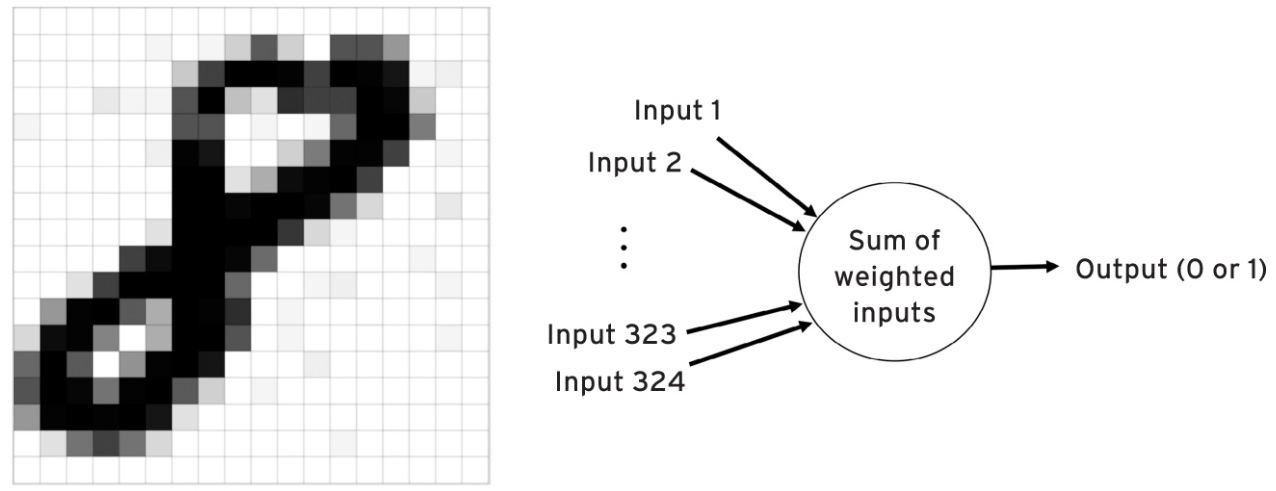
\includegraphics[width = 9cm]{images/perceptron1.png}
\end{center}

\vspace{-3mm}

\tiny \hfill \color{gray}Illustration: M. Mitchell \color{black}

\footnotesize

\begin{block}{Rosenblatt's perceptron}
\begin{itemize}
\item Inputs (pixel intensities) with weights
\item Nodes with activation levels from 0-1
\item (Perhaps) 0-1 output based on a threshold
\end{itemize}
\end{block}
\end{frame}

\begin{frame}{Word2vec}
\protect\hypertarget{word2vec-2}{}
\begin{center}
 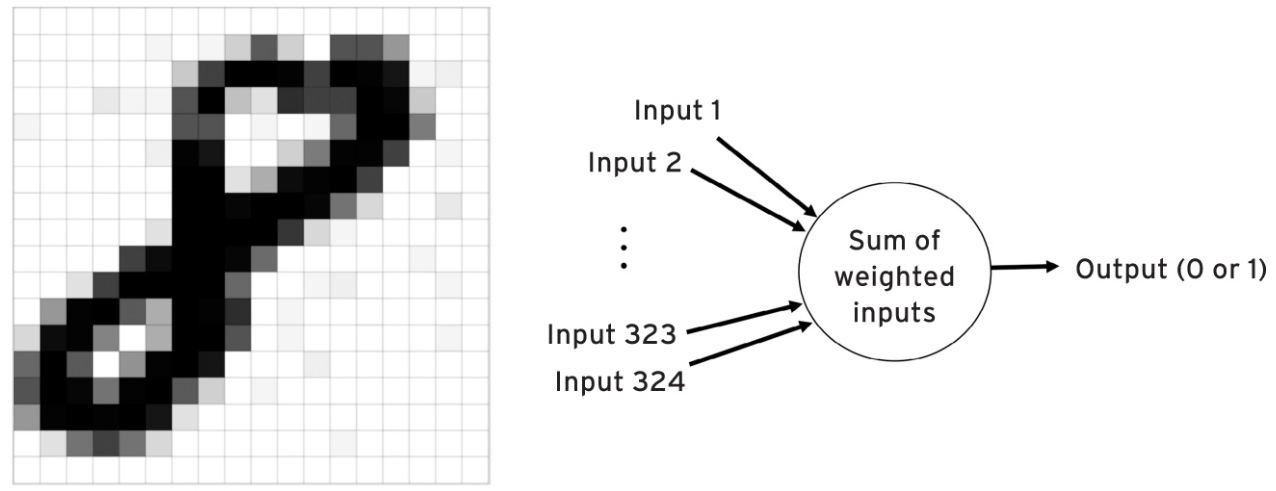
\includegraphics[width = 9cm]{images/perceptron1.png}
\end{center}

\vspace{-3mm}

\tiny \hfill \color{gray}Illustration: M. Mitchell \color{black}

\footnotesize

\begin{block}{Learning}
\begin{itemize}
\item Start with random weights
\item Test on a case:
\begin{itemize}
\item If right, don't change weights.
\item If wrong, change weights a bit, with focus on the ones more responsible for the judgment:
\begin{align*}
w_j & \leftarrow w_j = \overbrace{\eta}^{\text{learning rate}}(\underbrace{t}_{\text{correct output}} - \overbrace{y}^{\text{actual output}})\underbrace{x_j}_{\text{actual input}}
\end{align*}
\end{itemize}
\end{itemize}

\end{block}
\end{frame}

\begin{frame}{Word2vec}
\protect\hypertarget{word2vec-3}{}
\begin{columns}
\column{0.45\linewidth}
    
    

\begin{center}
 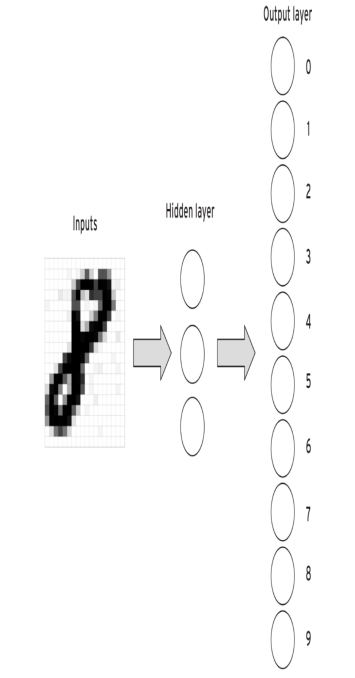
\includegraphics[height = 6cm, width = 5cm]{images/perceptron2.png}
\end{center}


\vspace{-3mm}
\tiny \hfill \color{gray}Illustration: M. Mitchell \color{black}



\column{0.5\linewidth}

\footnotesize 

\begin{itemize}
\item Each hidden unit takes a weighted sum of 324 inputs and passes on its activation level as input to outer layer units. 

\item Activation levels of outer layers are interpreted as network's levels of confidence in a classification problem.

\item Learning: back-propagation (gradient descent: approximate  the direction of steepest descent in the error surface w.r.t to weights, modify accordingly).
\end{itemize}

\end{columns}
\end{frame}

\begin{frame}{Word2vec}
\protect\hypertarget{word2vec-4}{}
\begin{block}{Distributional semantics}
\protect\hypertarget{distributional-semantics}{}
\begin{itemize}
\item "You shall know a word by the company it keeps" (John Firth, 1957)


\item "the degree of semantic similarity between two linguistic expressions $A$ and $B$ is a function of the similarity of the linguistic contexts in which $A$ and $B$ can appear." (A. Lenci, 2008)


\end{itemize}

\pause

\begin{center}
 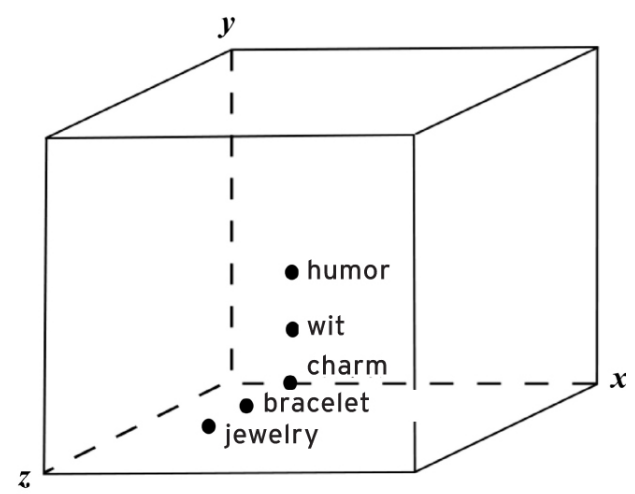
\includegraphics[height = 5cm, width = 5cm]{images/similarity1.png}
\end{center}

\vspace{-3mm}

\tiny \hfill \color{gray}Illustration: M. Mitchell \color{black}
\end{block}
\end{frame}

\begin{frame}{Word2vec}
\protect\hypertarget{word2vec-5}{}
\begin{block}{Google and Mikolov}
\protect\hypertarget{google-and-mikolov}{}
\emph{Efficient Estimation of Word Representation in Vector Space}, 2013

Let's train a neural network and use vectors of weights!

\begin{center}
 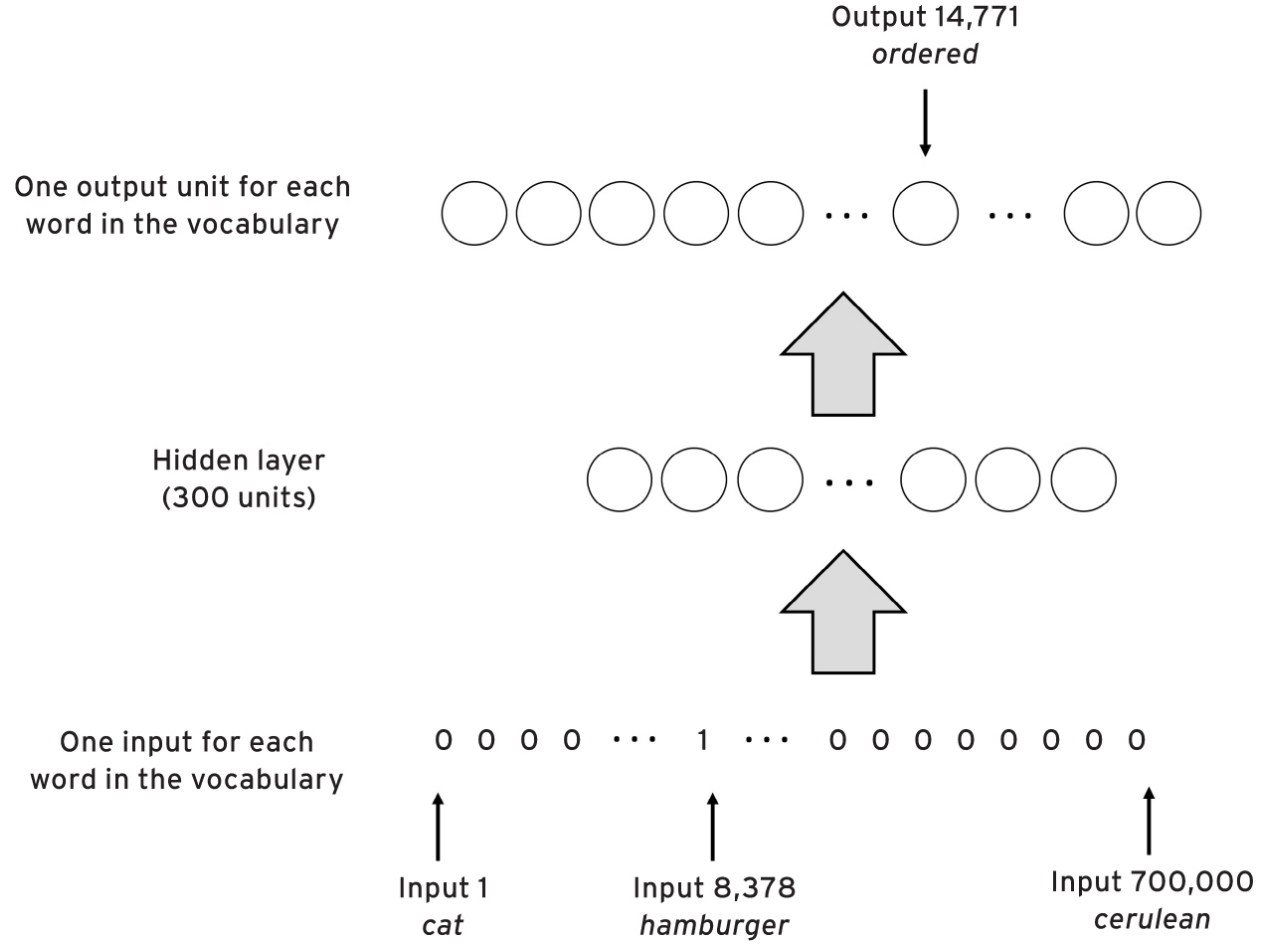
\includegraphics[height = 5cm, width = 6cm]{images/word2vec1.png}
\end{center}

\vspace{-3mm}

\tiny \hfill \color{gray}Illustration: M. Mitchell \color{black}
\end{block}
\end{frame}

\begin{frame}{Word2vec}
\protect\hypertarget{word2vec-6}{}
\begin{block}{Google and Mikolov}
\protect\hypertarget{google-and-mikolov-1}{}
\emph{Efficient Estimation of Word Representation in Vector Space}, 2013

Let's train a neural network and use vectors of weights!

\begin{center}
 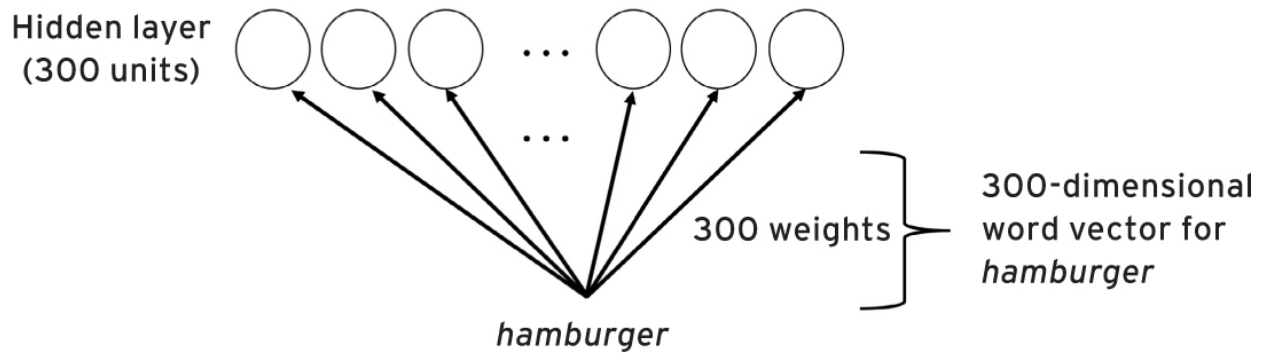
\includegraphics[height = 3cm, width = 7cm]{images/word2vec2.png}
\end{center}

\vspace{-3mm}

\tiny \hfill \color{gray}Illustration: M. Mitchell \color{black}
\end{block}
\end{frame}

\begin{frame}{Word2vec}
\protect\hypertarget{word2vec-7}{}
\begin{block}{Nearest words}
\protect\hypertarget{nearest-words}{}
\begin{itemize}
\item \textbf{philosophy}: philosophies, credo, ethos, principles, ethic, tenets, mantra, ideology, mindset, worldview

\item \textbf{sandwich}: sandwiches, burger, chicken sandwich, cheeseburger, burrito, burgers, pizza, turkey sandwich, hamburger, burritos
\end{itemize}

\pause
\end{block}

\begin{block}{Some similarities from \emph{philosophy}}
\protect\hypertarget{some-similarities-from}{}
Logic (.47), Nietzsche (.32), Hegel (.32), analytic (.13), burger (.08),
continental (.04), Russell (.04)
\end{block}
\end{frame}

\end{document}
